 \documentclass[12pt]{extbook}

\usepackage[T1]{fontenc}
\usepackage [utf8]{inputenc} 
\usepackage[spanish]{babel}
\usepackage{graphicx}	
\usepackage[unicode=true]{hyperref}

\begin{document}
\title{EXPERIENCIAS OBTENIDAS EN EL CURSO DE LENGUAJES DE PROGRAMACION}\maketitle
\begin{center}
\begin{description}
\item [{INDICE}]~
\item [{OBEJTIVOS...........................................................................3}]~
\item [{INTRODUCCION..................................................................4}]~
\item [{CAPITULO}] 1
\item [{Latex.......................................................................................6}]~
\item [{CAPITULO}] 2
\item [{Android..................................................................................10}]~
\item [{CAPITULO}] 3
\item [{Phyton....................................................................................16}]~
\item [{CAPITULO}] 4
\item [{Haskell....................................................................................22}]~
\item [{ANEXOS................................................................................24}]~
\item [{BIBLIOGRAFIA.....................................................................25}]~
\end{description}


\newpage

\title{OBJETIVOS}\maketitle
\end{center}


El principal objetivo dentro de la materia de Lenguajes de Programación
era el obtener experiencias en nuevos lenguajes y en nuevas plataformas,
para esto nuestro profesor guía nos dio a conocer cada uno de ellos,
en el curso se implanto los lenguajes que se aprenderían en el transcurso
del curso son:\\

\textbullet{} Android 

\textbullet{} Phyton 

\textbullet{} Haskell\\

Para cada uno se dedicara un capitulo dentro de este pequeño libro.
Ademas de esto implementaremos una manera de presentar nuestros trabajos
sin necesidad de utilizar los que son los productos de office, este
nuevo programa a usar es \LaTeX, se dedicara el primer
capitulo a las experiencias obtenidas al usar este tipo de programa,
además de los problemas que se tuvo que enfrentar en cada uno de los
proyectos dados.\\ Otro de los objetivos de esta materia es el uso de
un gestor de versionamiento, para esto se manejara el servidor del
GitHub, que nos permitira guardar avances de cada uno de nuestros proyectos
esta herramienta nos sera de mucha ayuda para no perder la informacion y
actualizarnos en cuanto a los avances que hace cada compañero del grupo.


\newpage
\begin{center}
\title{INTRODUCCION}\maketitle
\end{center}


Este trabajo es hecho por un estudiante del curso de Lenguajes de
Programacion, donde se da a conocer al lector posibles desafíos que
se tendrán que enfrentar dentro de la elaboración de los proyectos
de cada uno de los lenguajes mencionados en los objetivos de este
libro, para cada uno de estos se tuvo que buscar mucha ayuda de los
tutoriales ya que es nuevo para cada uno de nosotros el uso de estos
lenguajes, la experiencia que aportaba cada uno de estos para nuestras
vidas era cada vez mas contribuyentes ya que se aprendían nuevas cosas
con cada lenguaje, pero lo que mas se debe dar es el trabajo en equipo,
los grupos conformados deben trabajar juntos para poder realizar un
excelente trabajo y no sea muy pesado esto para uno, cosas que se
deben implantar desde que se crean estos, ya que es un trabajo en
grupo, necesitamos estar en contacto o subir los avances de cada uno
para poder mantenernos actualizados y permitirnos hacer cambios, ya
que una ves presentados los proyectos, es cuestión de cada uno avanzar
y mejorar estos para dar una mejor presentación para el usuario aquí
entra el versionamiento de la aplicación, para poder realizar esto
trabajamos con GitHub. \\

Para cada uno de estos se tratara un capitulo de estos y espero sea
de su agrado. 
\chapter{\LaTeX{}}
\LaTeX   Una de las herramientas que fuimos encomendados a aprender fue
el manejo de \LaTeX para realizar nuestras presentacion de nuestros
manuales de proyectos en la materia de Lenguajes de Programación,
fue una experiencia enriquecedora ya que pude observar con esta herramienta
muchas maneras de presentar y mejorar la presentación de un documento,
la utilidad de \LaTeX  para la creación de documentos de manera dinámica,
debido a su interfaz y su manera de manejarlos, tuvimos ciertos inconvenientes
como realizar la presentación de cada uno de ellos, podemos verlo
como un lenguaje mas, ya que  \LaTeX es un poco de sentencias que nos
permiten realizar ciertas maniobras en los documentos, como por ejemplo
al momento de colocar una imagen, esta requiere una sentencia y una
librería para poder ser colocada en el documento, además que requiere
dimensiones y posicionamiento, ciertas opciones dentro del ámbito
de \LaTeX permiten categorizarlo como una gran herramienta de desarrollo
de presentación sean estas guias, libros, artículos entre otras opciones
de presentar este documento.\\

Gracias a la colaboración de nuestro grupo de trabajo se puedo realizar
con éxito el aprendizaje de este nuevo lenguaje podríamos llamarlo
así, tanto en la revistas o papers publicados en la web, la información
para el uso de esta herramienta es de gran ayuda, se compensan de
la una a la otra, nuestro primer problema a enfrentar fue la creación
de un nuevo documento del tipo beamer, el cual fue nuestra primera
presentación para el proyecto del primer parcial de Lenguajes de Programación,
en el cual se debía realizar una presentación con beamer abarcando
la información sobre lo que iba a ser nuestro proyecto en Android,
el siguiente capitulo encontraremos la información sobre este proyecto,
nuestra presentación debía contar con la información solicitado por
nuestro profesor guía y lo cual listaremos:\\
 
\textbullet{} Titulo del Proyecto\\

\textbullet{} Descripción del Proyecto\\

\textbullet{} Ventajas\\

\textbullet{} Imágenes de la posible aplicación\\

Para cada ítem puesto anteriormente se tuvo ciertos problemas para
aplicarlos y presentarlos de manera adecuada, viendo que nosotros
no teníamos conocimiento de este tipo de documento, la búsqueda fue
nuestra única manera de aprender a manejar este tipo de documentos,
una vez teniendo los conocimientos básicos, solo fue cuestión de practicar
para poder obtener todos los conocimientos necesarios. \\

La presentación de las cabeceras, la centralización de las imágenes
y la justificación del texto fueron nuestros siguientes problemas
a enfrentar en la elaboración de este trabajo, fue un arduo trabajo
el tratar de conseguir los comandos respectivos para realizar lo pedido,
ya que ciertos resultados obtenidos no siempre eran los esperados,
solo fue necesidad de paciencia y perseverancia para poder obtener
la información necesaria, una vez que este obstáculo fue atravesado
estuvimos dispuestos a enfrentar cualquier otro.\\

GitHub, es una forma de manejar el versionamiento de las aplicaciones, que nos permite
guardar los nuevos cambios de cada una de ella, teniendo en cuenta
los antiguos cambios, es una herramienta que nos permitirá mantenernos
actualizados todos los compañeros de grupo, además que nos permitirá
en que ha trabajo cada uno para ponerle atención a los cambios realizados
para cada uno, el uso de esta herramienta para estos trabajos fue
de mucha ayuda para saber la colaboración de cada uno de los integrantes
del grupo. \\


\begin{center}
\title{CONCLUSIONES}\maketitle
\end{center}

El trabajo en equipo para la elaboración del cualquier tipo de documento
en la herramienta de latex fue muy divertido y recreativo, el punto
clave en la elaboración de los documentos es la imaginación de cada
uno para hacer una fantástica presentación, la experiencia obtenida
de este proyecto a más de interesante fue de mucha importancia ya
que con esto vemos la posibilidad de generar otro tipo de presentación
de una manera mas presentable, mas estética para su posterior publicación,
un logro obtenido en este capitulo fue el aprendizaje de este tipo
de documento. Una desventaja que se podría recalcar para la utilización
de este tipo de documentos es el uso de líneas de código para la implementación
del texto, aunque no hay que negar que los resultados después de haber
aplicado las mismas sean increíbles, es recomendable para los futuros
usuarios de este material, instruirse bien y practicar bastante, usar
la imaginación que tienen para un diseño espectacular.\\

Ademas de \LaTeX, el github fue una gran experiencia
el poder usarlo, esta herramienta es de gran apoyo para un desarrollador
de software, ya que los versonamientos son muy importantes para saber
las mejoras que se deben hacer en los programas, viendo los nuevos
usos que se le puede dar a la tecnología y lo que se le puede aplicar
a nuestra aplicación, la aplicación para nuestros programas fue de
vital importancia para el profesor, ya que con esto podría ver la
colaboración de cada uno para el proyecto.
\chapter{ANDROID}
\begin{center}
\title{\Large{DRIVER SAFE}}\maketitle
\end{center}
\begin{center}

\includegraphics[width=7cm]{driversafe.jpg}
\end{center}
El primer proyecto a presentar fue una aplicación para dispositivos
android, para el cual nos pedia que se le diera un uso y sea este
un beneficio que no este prestando alguna otra persona, para esto
pensamos en lo que mas esta sufriendo la gente, en lo que menos se
percata, llegando a una conclusión, en el momento de conducir a veces
sobrepasa la velocidad limite establecida incluso las señalizaciones,
para esto pensamos en crear una aplicación que les permita tener en
cuenta todas esas pequeñas infracciones que cometen sin darse cuenta,
que luego pueden convertirse en un gran problema, esta aplicación
seria de una gran ayuda ya que nos advertiría el momento de cometer
una infracción.
\newpage
\begin{center}
\title{MANUAL DE USUARIO}\maketitle
\end{center}
Driver Safe es una aplicación elaborada por los estudiantes de Lenguajes
de Programación para los usuarios que posean autos y no desearían
ser infraccionados, esta aplicación esta pensada con la finalidad
de hacer que el usuario se mas precavido al momento de conducir, consta
de 3 pantallas que se planteara una a una que representa: \\
\subsection*{VELOCIMETRO}


\begin{center}
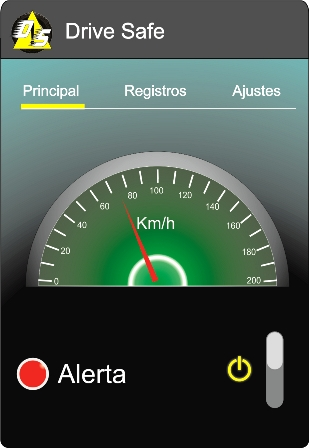
\includegraphics[width=7cm]{principal.jpg}
\end{center}

La primera ventana de nuestra aplicación consta de la imagen del velocímetro
que marcara la velocidad actual del vehículo, contiene además de un
botón de alerta que nos avisara el momento en el cual el usuario rebase
la velocidad establecida por seguridad vial, este ventana consta con
la activación del GPS ya que es la única que de obtener los datos
instantáneos y actuales desde el dispositivo, una vez que el GPS capte
la velocidad del vehículo y compare la velocidad establecida por la
zona en la que transita, esta activara el botón de alarma en caso
de ser necesario, el otro botón que tenemos en la parte inferior nos
permitirá apagar o encender el equipo, ya que esta aplicación trabaja
con la tecnología GPS hace que la batería del dispositivo baje rápidamente.

\subsection*{REGISTRO}

\begin{center}
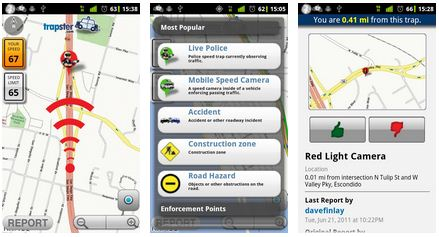
\includegraphics[width=7cm]{registro.jpg}
\end{center}

Esta ventana guardara todas las infracciones que hemos cometido durante
el viaje, esta pestaña de nuestro programa, registrara tanto los excesos
de velocidad, el paso de semáforos, toda clase de posibles infracciones
que puedes ser registradas por los satélites del gps, la pestaña anterior
se basa en esta para la función del botón de alarma, que hace que
esta se encienda cuando vuelva a cometer una infraccion en la misma
zona, con el objetivo de que no vuelva a cometer lo mismo.\\

La información que se guardara en cada registro sera: \\

\textbullet{} Direccion\\

\textbullet{} Velocidad registrada en el momento\\

\textbullet{} Fecha y Hora \\

\begin{center}
\subsection*{AJUSTES}
\end{center}

\begin{center}
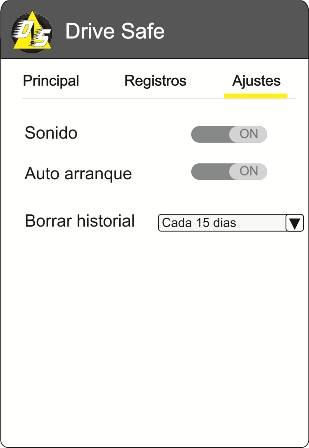
\includegraphics[width=7cm]{ajustes.jpg}
\end{center}

La ultima pestaña de nuestro programa es la de ajustes, a veces el
sonido de la aarma puede ser un poco molesta, para esto se añadió
un botón para activar y desactivar el sonido, además, esta aplicación
cuenta con la opción para desactivar el autoarranque, ya que nuestra
aplicación una vez instalada, esta no es necesaria que la abran desde
su icono, se activa sola pero a veces el usuario no desea que esta
aplicación consuma batería o no conducirá, este botón hara que la
aplicación deje de activarse cada que se encienda el dispositivo.
A veces el historial es tan antiguo que ya no es necesaria esa información,
para eso esta la opción de borrar historial, tendrá destinado borrar
hasta cierta cantidad de días atrás.

\begin{center}
\title{CONCLUSIONES}\maketitle
\end{center}

Manejar el lenguaje android para este crear aplicación para dispositivos
que son actuales fue una gran experiencia ya que de alguna u otra
manera, este tipo de aplicaciones son las que mas saldrán al mercado
con el avance de la tecnología, este lenguajes en cuanto a codificación
contiene un gran parecido a Java, se trabajo en Eclipse con una plataforma
de android la cual nos haría experimentar en este lenguaje, el establecer
una relación de compañerismo hara que este trabajo sea mas divertido
y se genere una lluvia de ideas que permite que colaboremos con excelentes
maneras de solucionar ciertos problemas.\\

El manejar este lenguaje de programación contaria como una actualización
a la información y nuevas generaciones de lenguajes, cada vez que
salen nuevos lenguajes para programar estos se parecen mas al lenguaje
común, eso permite a los programadores que puedan entender de manera
mas veloz la manera en la que se programa, además que el trabajo en
grupo es de bastante apoyo, ya que mientras el uno trabaja en una
parte del proyecto el otro puede continuar en otra parte o realizar
búsquedas de información para poder continuar de una manera rápida. 

\chapter{PHYTON}
\begin{center}
\title{\Large{QUIEN SABE, SABE!!!}}\maketitle
\end{center}

\begin{center}

\includegraphics[width=5cm]{quienquieresermillonario.jpg}
\end{center}

Nuestra segundo proyecto a presentar fue una idea del profesor realizarla
en phyton, para lo cual nos pidió que este sea para el uso de personas
no videntes, lo cual seria una aplicación solo en audio, ya que los
no videntes cuentan con un teclado especial para saber que teclas
presionar, esto les facilitara el uso de la aplicación. 

Nuestro primer reto a enfrentar fue el pensar que aplicación realizar
para este tipo de pedido que nos realizaba nuestro profesor, en una
lluvia de ideas encontramos una posible solución para esto, la creación
de un juego basado en el programa de televisión \textquotedblleft{}Quien
quiere ser Millonario\textquotedblright{}, pero en versión politécnica,
\textquotedblleft{}Quien sabe, sabe!!!\textquotedblright{}. 
\newpage
\begin{center}
\title{MANUAL DE USUARIO}\maketitle
\end{center}

Nuestro programa presentara por pantalla lo siguiente:\\

\begin{center}
\includegraphics[width=12cm]{principal1.jpg}
\end{center}

El programa le dara las indicaciones que debidas para su propio uso,
iniciando con el titulo de programa y las teclas que debe presionar
para accesar a cada una de las opción mostradas por pantalla, como
son:\\

J: Jugar\\

I: Instrucciones \\

A: Autores \\

S: Salir \\

Al momento de seleccionar cada una de estas letras se nos abrirá una
nueva ventana veremos que se presentara en cada uno de ellos, y la
modalidad en la que nos dará las opciones a presionar. \\

Para la opción J se presentara en pantalla:\\

\begin{center}
\includegraphics[width=12cm]{jugar.jpg}
\end{center}

Una de las 19 preguntas que se generaran de manera aleatoria para
el usuario, cada una de ellas sera relatada junto con sus opciones,
A,B,C,D, las cuales deben ser presionadas por el usuario, para poder
ganar el juegos este debe acertar a 15 de ellas, cada respuesta acertada
generara una cantidad de puntos, el tiempo fue un problema ya que
no encontrábamos la manera de encerarlo asi que solo se podía añadir
al tiempo anterior el nuevo tiempo de la siguiente pregunta, una vez
que el usuario no acierte una pregunta el juego acabara presentado
la cantidad de puntos que gano.\\

Para poder realizar la selección de nuestras opciones, el programa
le hablara al usuario cada una de ellas y solo debe presionar la tecla
correcta sin necesidad de presionar un enter, además en caso de que
el usuario sea vidente no es necesario que presione la tecla, puede
ser uso del mouse para esta selección. \\
\newpage
Para la selección de la tecla I se mostrara por pantalla:\\
\begin{center}
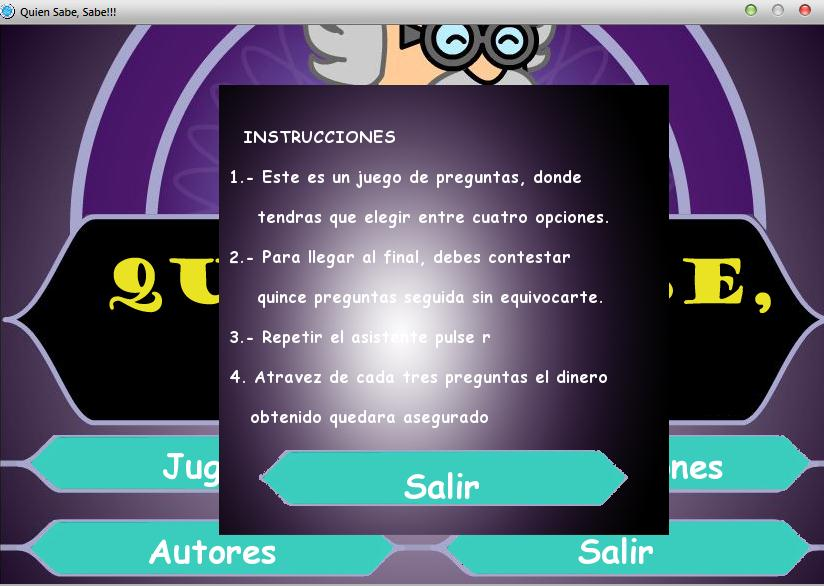
\includegraphics[width=12cm]{instrucciones.jpg}
\end{center}
Aquí mostrara para los usarios videntes lo de manera escrita las instrucciones
del juego y además para los usuario no videntes podrán escuchar lo
que esta escrito, al igual para salir de esta opción tiene un botón
Salir, que podrá ser accesado mediante el mouse o presionando la tecla
S, que también se le mencionara al usuario como entrar a ella, esta
opción no contiene mucho que hacer, simplemente se escucha lo que
se deberá hacer dentro del juego y en cierta manera como aprovechar
estos beneficios de tal.\\
\newpage
Para la opción A se mostrara por pantalla:\\
\begin{center}
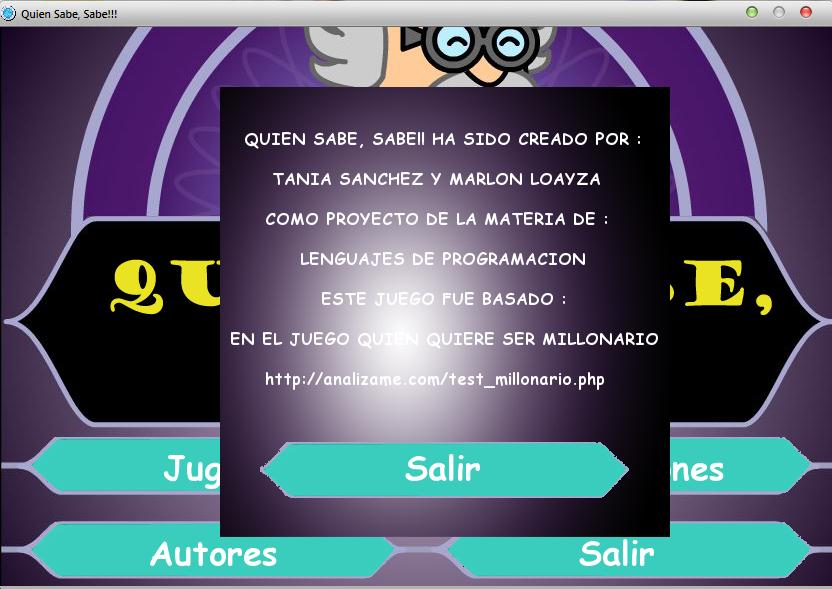
\includegraphics[width=12cm]{autores.jpg}
\end{center}
Esta opción de nuestro juego, dara una breve descripción del objetivo
del juego, incluyendo cuales fueron los autores del juego, igual que
en las ventanas anteriores sera disponible para personas videntes
y no videntes. Por ultimo tenemos la opción de salir de nos hara salir
del juego\\

\begin{center}
\title{CONCLUSIONES}\maketitle
\end{center}

La experiencia obtenida por este lenguaje como fue puesta en la introducción
fue diferente a la de Android, al ser un lenguaje diferente este también
tiene sus diferencias en cuanto a sintaxis de codificación, para lo
cual se tuvo que buscar ayuda de la web para poder realizar este trabajo,
nuestro primer reto a enfrentar fue el sonido para incorporarlo al
programa, y como se trabajaría con el sonido, para esto tuvimos la
ayuda de un programa que me permite dado un texto, hablarlo y grabarlo
en formato ogm que nos permitiría leer nuestro programa al momento
necesario para la presentación de cada ventana y pregunta, una vez
solucionado el problema de audio, fuimos a nuestro siguiente obstáculo
que era aprender los sintaxis para la creación de funciones y la implementación
de estos sonidos para que se reproduzcan dentro del programa, ya que
teníamos todo enfocado, solo disponíamos del tiempo suficiente para
poder realizar, fue un trabajo muy duro pero divertido de hacer, el
trabajo en equipo es indispensable para este tipo de proyectos, el
desarrollo en este lenguaje al aprender a manejarlo nos daremos cuenta
que no es complicado pero cuando todo es nuevo siempre tendremos dificultades.

\chapter{HASKELL}
\begin{center}
\title{\Large{MASTERMIND}}\maketitle
\end{center}

\begin{center}
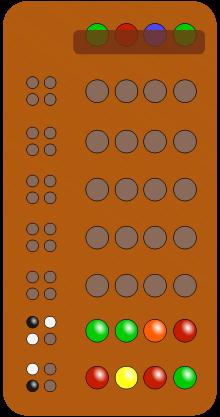
\includegraphics[width=4cm]{mastermind.jpg}
\end{center}
El último lenguaje en aprender fue el haskell, tiene diferencias a
los demás lenguajes en el sentido que es funcional, las sintaxis son
diferentes, cosas nuevas se aprenderán para este capitulo, en cuanto
al programa pedido por nuestro profesor guía fue Mastermind: \\


El juego se basa en dado un conjunto de 4 bolitas con colores en cierta
posición dada por el computador, el jugador debe acertar la posición
correcta del cada una de estas bolitas acertando también en su color,
para saber si hemos puesto bien cada una de ellas, a lado de la posición
de que es puesta por el jugador, este tendrá en cuenta que hay 4 bolitas
mas con colores lo cual nos indicara si la posición y color están
correctos, a continuación mostraremos como se identificara cada posición:\\
\begin{center}
1          2\\

4          3\\	 
\end{center}
Las posiciones que están anteriormente indican cual es la bolita correcta
con el color correcto, se nos pintaran los siguientes 2 colores: \\

BLANCO: Indica que el color esta correcto pero no la posición. \\
	
NEGRO: Indica que tanto el color como la posición es correcta. \\

El usuario tiene hasta 7 oportunidades para poder terminar el juego
, en esencia ese es todo el juego, nuestro trabajo es analizar uno
de los 2 algoritmos enviados por el profesor guía, de modo que en
el juego trabajemos con alguno de ellos, a pesar de que este tipo
de lenguaje funcional es muy diferente a los demás, el esfuerzo por
cada compañero para tratar de programar en aquí es demasiado grande.

\begin{center}
\title{CONCLUSIONES}\maketitle
\end{center}

Este es un gran reto que todavía estamos tratando de vencer, ya que
este tipo de lenguaje funcional es muy diferente a los que normalmente
solemos aplicar, una ves terminado este proyecto implementaremos el
manual de usuario del mismo, para poder concluir con este pequeño
libro sobre las experiencias de usar todos estos lenguajes para nuestros
proyectos.
\newpage
\begin{center}
\title{ANEXOS}\maketitle
\end{center}
En esta sección anexaremos los codigos hechos para el lenguaje de Phyton
como para Android, el codigo de Haskell tan pronto este terminado, podra ser
accesado:\\

\large{PHYTON}\\
\href{https://www.dropbox.com/s/aj9wth4m2b21y71/Sabeee.rar}{https://www.dropbox.com/s/aj9wth4m2b21y71/Sabeee.rar}
\large{ANDROID}\\
\href{https://www.dropbox.com/s/9mvtnapx25ixffd/DriveSafe.rar}{https://www.dropbox.com/s/9mvtnapx25ixffd/DriveSafe.rar}

\newpage
\begin{center}
\title{BIBLIOGRAFIAS}\maketitle
\end{center}
\href{http://www.elandroidelibre.com/2010/08/aprendiendo-android-v-inicializacion-a-la-api-del-gps.html}{http://www.elandroidelibre.com/2010/08/aprendiendo-android-v-inicializacion-a-la-api-del-gps.html}\\
\href{http://codigojavaoracle.com/android-2/gps-con-android-mostrar-tu-posicion/}{http://codigojavaoracle.com/android-2/gps-con-android-mostrar-tu-posicion/}\\
\href{http://translate.google.com.ec/translate?hl=es&sl=en&u=http://yannesposito.com/Scratch/en/blog/Haskell-the-Hard-Way/&prev=/search\%3Fq\%3Dhaskell\%2Btutorial\%2Bblog\%26hl\%3Des\%26tbo\%3Dd\%26biw\%3D1163\%26bih\%3D580&sa=X&ei=eYEQUdqqKY_e8wSdqYH4Cw&ved=0CC4Q7gEwAA}{http://translate.google.com.ec/translate?hl=es\&{}sl=en\&{}u=http://yannesposito.com/Scratch/en/blog/Haskell-the-Hard-Way/\&{}prev=/search\%{}3Fq\%{}3Dhaskell\%{}2Btutorial\%{}2Bblog\%{}26hl\%{}3Des\%{}26tbo\%{}3Dd\%{}26biw\%{}3D1163\%{}26bih\%{}3D580\&{}sa=X\&{}ei=eYEQUdqqKY\_{}e8wSdqYH4Cw\&{}ved=0CC4Q7gEwAA}
\title{Marlon Vinicio Loayza Feijoo}
\end{document}